\section{Scheduling with Known Arrival Types: The WAIT Algorithm}
\label{sec:wait}

This section introduces the \textit{Waiting for Accumulated Inference Threshold} (WAIT) algorithm, a scheduling policy that maximizes throughput when prompt arrival types are known. Building on the fluid dynamics from Section \ref{sec:fluid}, WAIT optimizes batch formation by accumulating prompts until specific thresholds are met. This approach maintains the system near equilibrium, respecting memory constraints while optimizing latency and time-to-first-token (TTFT). We assume that the memory capacity $C\ge M^*,$ the equilibrium memory capacity given in \eqref{eq:memory_multi2} (otherwise the throughput can never approach the optimal fluid throughput \eqref{throughput_fluid_multiple} by Proposition \ref{prop::online policy expected throughput upper bound, multiple type}).

\begin{remark}[On the Assumption $C \geq M^*$]
\label{remark:memory_assumption}
Our theoretical analysis assumes $C \geq M^*$, as this is the necessary condition under which the system can achieve stable operation without accumulating backlog. When $C < M^*$ (the overloaded regime), our algorithms remain effective: the eviction prevention mechanism still outperforms baselines, as demonstrated in Section~\ref{sec:experiments}. Avoiding eviction cascades provides value across all operating regimes.
\end{remark}

\subsection{Motivation: Why Naive Scheduling Fails}
\label{subsec:wait_motivation}

We first demonstrate why naive scheduling policies fail even when memory capacity is sufficient, motivating the design of WAIT.

Consider what happens under a First-Come-First-Serve (FCFS) policy that processes prompts immediately upon arrival. Even when the memory capacity $C$ equals the equilibrium memory $M^*$---seemingly sufficient to handle the workload---FCFS can trigger catastrophic failure. The following proposition formalizes this observation.

\begin{proposition}\label{prop:lower_bound_FCFS}
When the memory capacity \(C\) equals the equilibrium memory \(M^*\), there exists an instance where the First-Come-First-Serve (FCFS) policy incurs a throughput gap of \(\throughput^* - \mathbb{E}[\throughput^T] = \Omega(1)\) as \(T \to \infty\).
\end{proposition}

The proof is provided in Appendix. To illustrate the mechanism behind this failure concretely, consider the following example.

\begin{example}[Eviction Cascade under FCFS]
\label{ex:fcfs_cascade}
Consider a single prompt type where each prompt is a simple query such as ``Hello'' with a 1-token response ``Hi''---prefill length $l=1$ and decode length $l'=1$. Each prompt occupies 1 unit of memory after prefill and 2 units after decode. Let the memory capacity be $C=12$ and arrival rate $\lambda=4$. The fluid equilibrium has 4 prompts at each stage (prefill and decode), using exactly $4 \times 1 + 4 \times 2 = 12$ units of memory with 4 completions per iteration.

Now suppose the system starts slightly imbalanced with 6 prompts at stage 0 (awaiting prefill) and 3 prompts at stage 1 (in decode). Under FCFS:
\begin{enumerate}
    \item \textbf{Iteration 1}: Process all 9 prompts. The 3 decode prompts complete, but the 6 prefill prompts advance to decode, requiring $6 \times 2 = 12$ units. Memory is exactly full with only 3 completions.
    \item \textbf{Iteration 2}: During iteration 1, approximately 4 new prompts arrive. To admit them for prefill ($4 \times 1 = 4$ units needed), we must evict 2 decode prompts (freeing $2 \times 2 = 4$ units). Now we have 4 prefill + 4 decode = $4 + 8 = 12$ units.
    \item \textbf{Iteration 3}: The 4 decode prompts complete (4 completions). The 2 previously evicted prompts, having lost their KV caches, must now restart from the prefill phase (stage $s=0$)---they re-enter the queue as new arrivals, competing for resources alongside genuinely new prompts. This restart mechanism perpetuates the imbalance.
\end{enumerate}
This eviction-restart cycle persists, yielding approximately 3-3.5 completions per iteration instead of the optimal 4. \textbf{Even though $C = M^* = 12$ (theoretically sufficient capacity), FCFS causes cascading failures that reduce throughput by 12-25\%.}
\end{example}

This example demonstrates a fundamental insight: \emph{memory sufficiency alone does not guarantee stability}---a system that should be stable can become unstable under poor scheduling. The root cause is that FCFS does not maintain \emph{load balance}: it admits prompts greedily, causing the system to deviate from the fluid equilibrium and triggering the eviction-restart cycle.

\subsection{The WAIT Algorithm}
\label{subsec:wait_algorithm}

The WAIT algorithm prevents eviction cascades by maintaining load balance through a threshold mechanism. The core idea is to control admission at each decode stage, ensuring that the rate of new arrivals matches the rate of completions. This keeps the system close to the fluid equilibrium derived in Section~\ref{sec:fluid}, \emph{approaching load balance} where arrival and completion rates match. This principle---maintaining the system near equilibrium through controlled admission---is central to preventing the cascading failures illustrated in Example~\ref{ex:fcfs_cascade}.

The threshold-and-wait mechanism achieves three goals: (1) prevents \emph{eviction cascades} by controlling admission; (2) \emph{decouples multi-type dynamics} into $m$ independent analyses, breaking inter-type dependencies through algorithm design; (3) \emph{exploits memory fully} by forming batches near equilibrium size $M^*$, treating memory as a resource to maximize throughput, not merely a constraint to satisfy.

\paragraph{Algorithm Description.} For each prompt type $j \in [m]$, WAIT sets a threshold $n_j$ derived from the fluid dynamics. At time $t$, the algorithm monitors the inventory $n_{js}^t$---the number of waiting prompts of type $j$ at stage $s$. Type $j$ prompts are included in a batch only when:
\[
n_{j0}^t \geq n_j.
\]
When this condition is met, WAIT constructs a batch by selecting $\min\{n_j, n_{js}^t\}$ prompts of type $j$ at each stage $s$ for all types meeting the threshold. If no type satisfies the condition, the algorithm waits for more arrivals. KV caches for waiting prompts are preserved, avoiding redundant computation. The complete specification is in Algorithm~\ref{alg:wait} and Figure~\ref{fig:wait}.

\begin{figure}
    \centering
    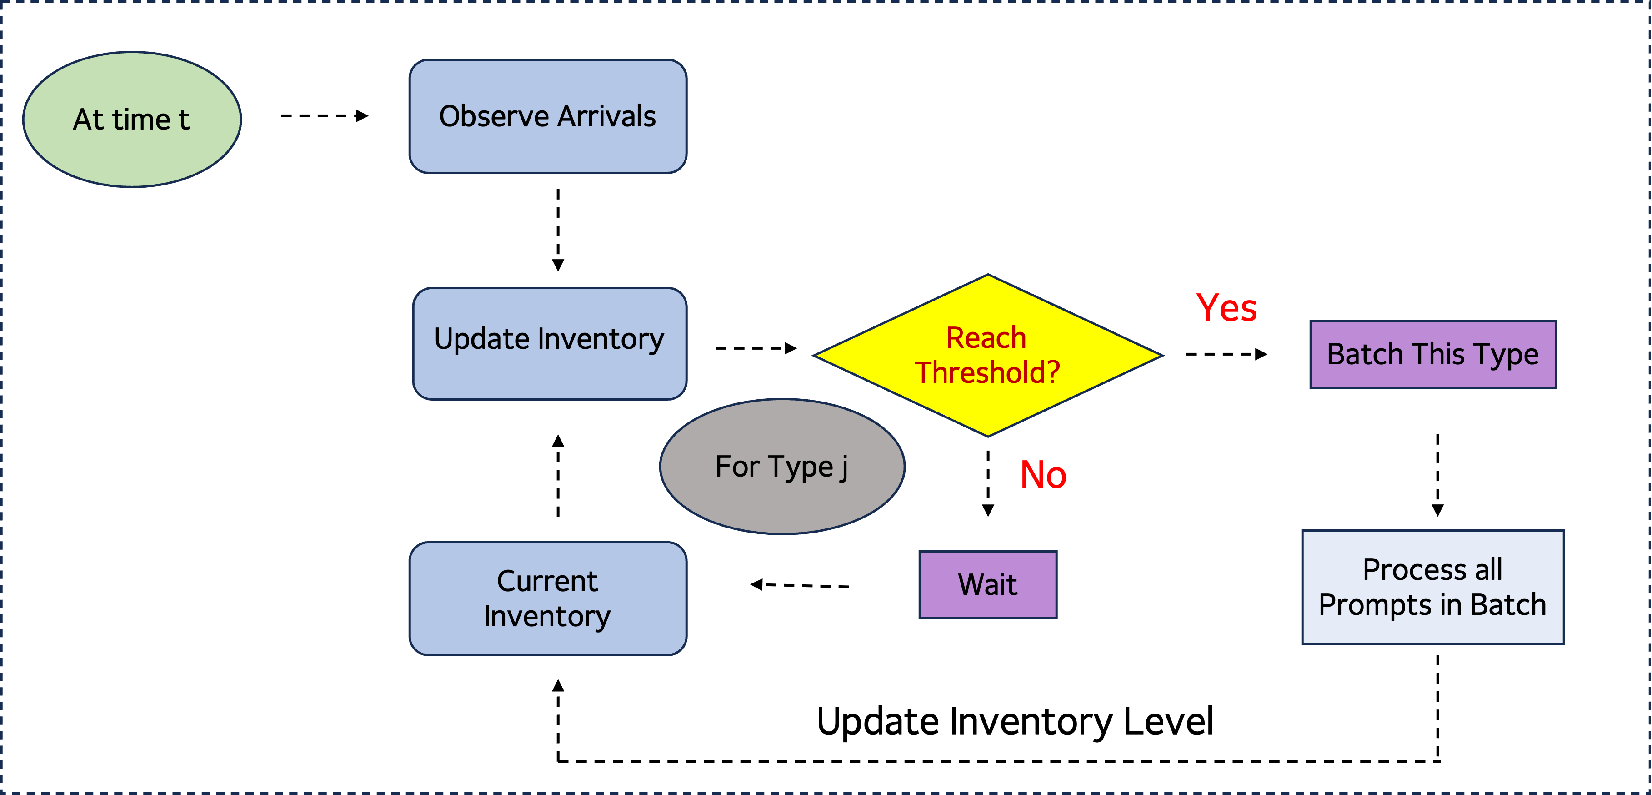
\includegraphics[width=0.9\linewidth]{Experiments_pdf/fig_WAIT.pdf}
    \caption{Pipeline of Algorithm \ref{alg:wait}}
    \label{fig:wait}
\end{figure}

\begin{algorithm}[h]
\caption{WAIT: Waiting for Accumulated Inference Threshold}
\label{alg:wait}
{\small\linespread{1.0}\selectfont
\begin{algorithmic}[1]
\Require Memory $C$, arrival rates $\lambda_j$, thresholds $n_j$ satisfying \eqref{eq:wait_thresholds}, $\forall j \in [m]$
\State Initialize prompt inventory $n_{js} \gets 0$ for all $j \in [m], s \in \{0, 1, \dots, l_j'\}$
\State Initialize event queue with arrival events for each type $j$
\State Set current time $t \gets 0$
\While{True}
    \State Wait for the next event (arrival or batch completion)
    \If{event is an arrival of type $j$}
        \State Update inventory: $n_{j0} \gets n_{j0} + 1$  \Comment{Add new prompt to waiting queue of prefill phase}
    \ElsIf{event is a batch completion}
        \State Update inventory: For each $j$ in batch $B$, $n_{js} \gets n_{js} - \min\{n_j, n_{js}\}$ for $s = 0, \dots, l_j'$
        \State Advance prompts: For each $j$, move $\min\{n_j, n_{js}\}$ prompts from stage $s$ to $s+1$
        \State Clear KV caches for prompts reaching stage $l_j' + 1$  \Comment{Free memory for completed prompts}
    \EndIf
    \State Check if $n_{j0} \geq n_j$ for any $j \in [m]$  \Comment{Check threshold for batching}
    \If{condition $n_{j0} \geq n_j$ is met for some $j$}
        \State Form batch $B$ by selecting $\min\{n_j, n_{js}\}$ prompts of type $j$ at each stage $s$ for all $j$ meeting the condition
        \State Process batch $B$, keep prompts outside the batch waiting and do not delete their KV caches
    \EndIf
\EndWhile
\end{algorithmic}
}
\end{algorithm}

\subsection{Asymptotic Analysis}
\label{subsec:asymptotic_analysis}
We evaluate the performance of WAIT in an asymptotic regime that captures long-run system behavior. Specifically, we scale the arrival rates to $\lambda_j^{(\zeta)} = \zeta \lambda_j$ and processing speeds accordingly ($(d_0^{(\zeta)},d_1^{(\zeta)})=(\zeta^{-1}d_0,\zeta^{-1}d_1)$) while keeping memory capacity $C$ fixed. This can equivalently be viewed as scaling the time horizon from $T$ to $\zeta T$ while keeping arrival rates and processing speeds unchanged. As $\zeta \to \infty$, we obtain infinite-horizon limits that characterize the system's long-run average performance, allowing us to study throughput stability under sustained load.

% and (ii) the \emph{many-server heavy traffic scaling}, where both arrival rates and memory capacity are scaled proportionally.

% \textbf{Conventional Heavy Traffic:} 

% \textbf{Many-Server Heavy Traffic:} Here, we scale arrival rates to $\lambda_j^{(\zeta)} = \zeta \lambda_j$ and memory capacity to $C^{(\zeta)} = \zeta C$, compressing the time horizon by a factor of $1/\zeta$ (i.e., observing over $[T]$). This regime examines system performance when both demand and resources grow proportionally.

\textbf{Performance Metric:} We focus on the average throughput, denoted $\throughput^{(\zeta, \pi)}$, where $\pi$ represents the WAIT policy, defined as:
\[
\throughput^{(\zeta, \pi)} = \frac{1}{\zeta T} \sum_{j=1}^m N_j^{(\zeta, \pi)},
\]
with $N_j^{(\zeta, \pi)}$ being the total number of type-$j$ tokens processed under scaling $\zeta$. The average latency $\Latency^{(\zeta,\pi)},\TTFT^{(\zeta,\pi)}$ and TTFT are defined similarly by dividing the quantity by $\zeta$. Our objective is to demonstrate that $\throughput^{(\zeta, \pi)}$ approaches the fluid equilibrium benchmark $\throughput^* = \sum_{j=1}^m \lambda_j l_j'$ (\ref{throughput_fluid_multiple}) as $\zeta \to \infty$ while giving bound to the latency and TTFT.

\subsection{Theoretical Analysis}
\label{subsec:main_theorem}
When memory capacity satisfies \(C \geq M^*\) (where $M^*$ is the equilibrium memory from Equation~\eqref{eq:memory_multi2}), consider the WAIT policy \(\pi\) parameterized by thresholds \([n_1, \dots, n_m]\), where \(n_j\) is the threshold for type-$j$ prompts at each stage. WAIT is asymptotically optimal when the thresholds satisfy:
\begin{equation}
\label{eq:wait_thresholds}
\begin{aligned}
\Delta T(n_{1:m}) &:= d_0 + d_1 M^{\pi} \leq \tfrac{n_j}{\lambda_j},\, \forall j\in[m],\\
 M^{\pi} &= \sum_{j=1}^m n_j (l_j' + 1) \big(l_j + \tfrac{l_j'}{2}\big)
\end{aligned}
\end{equation}
The intuition follows from Equation~\eqref{eq:time_fluid}: when type $j$ is included in a batch, the iteration time $\Delta T$ ensures that expected arrivals of type $j$ do not exceed $n_j$. This keeps the system close to the fluid equilibrium, using memory capacity fully for throughput while avoiding overflow.

% we obtain the policy class $\Pi$, each $\pi = [n_1,\cdots,n_m]\in \Pi$ with corresponding memory capacity $M^{\pi} \geq  M^*$.

% $\forall \pi \in \Pi$, when prompts of all $m$ types are in the same batch, $\text{Arrival}_j\leq \text{Completion}_j$. Indeed, when type $j$ is in the batch, no matter what the other types are in the batch, we have that $\text{Arrival}_j\leq \text{Completion}_j$. Specifically, when $M^c = M$, the policy is $\pi = [ \frac{n_1^*}{l_1^\prime+1},\,\cdots,\,\frac{n_m^*}{l_m^\prime+1} ]$. 

% The following theorem establishes the near-optimality of WAIT under heavy traffic conditions.
\begin{theorem}
\label{thm:wait_heavy_traffic}
    Assume the thresholds $\pi=[n_1,\dots,n_m]$ satisfy \eqref{eq:wait_thresholds}, then we have 
% \begin{equation*}
%     \begin{aligned}
%         &\throughput^*-\ex{}{\throughput^{(\zeta,\pi)}}=O((\zeta T)^{-\frac{1}{2}}),\\ 
% &\ex{}{\Latency^{(\zeta,\pi)}}=O\prn{(\zeta T)^{\frac{1}{2}}},\\
% &\ex{}{\TTFT^{(\zeta,\pi)}}=O\prn{(\zeta T)^{\frac{1}{2}}}.
%     \end{aligned}
% \end{equation*}
$$
\begin{aligned}
    &\throughput^*-\ex{}{\throughput^{(\zeta,\pi)}}=O((\zeta T)^{-\frac{1}{2}}),\\ 
&\ex{}{\Latency^{(\zeta,\pi)}},\,\ex{}{\TTFT^{(\zeta,\pi)}}=O\prn{(\zeta T)^{\frac{1}{2}}}.
\end{aligned}
$$
    Moreover, when we have $\Delta T_{[1,\dots,m]}<n_j/\lambda_j,\forall j\in[m]$ where $\Delta T_{[1,\dots,m]}$ is defined in \eqref{eq:wait_thresholds}, it holds that
$$    \begin{aligned}
        &\throughput^* - \ex{}{\throughput^{(\zeta,\pi)}} = O(1/(\zeta T)), \\ 
&\ex{}{\Latency^{(\zeta,\pi)}},\, \ex{}{\TTFT^{(\zeta,\pi)}} = O(1).
    \end{aligned}$$
\end{theorem}



% \begin{theorem}
% \label{thm:wait_heavy_traffic}
% Under the conventional heavy traffic regimes, the WAIT algorithm achieves near-optimal throughput. Specifically:
% % \begin{itemize}
% %     \item In the many-server heavy traffic regime:
% %     \[
% %     \liminf_{\zeta \to \infty} \zeta^{-1} \mathbb{E} \left[ \throughput^{\zeta, \pi} \right] \geq (1 - T^{-1}) \throughput^*,
% %     \]
% %     where the time horizon is $T$.
% % \end{itemize}
% when $C = M^*$, we have that $\pi = [\frac{n_1^*}{l_1^\prime+1},\,\cdots,\, \frac{n_m^*}{l_m^\prime+1}]$. This is a special case where all types satisfy the condition $\Delta T_{[1,\cdots,m]} = \frac{n_j}{\lambda_j}$. So with the union bound, we have the expected upper bound of the throughput gap to the $\text{Throughput}^*$ under the fluid system \gan{ref, and the prop~\ref{prop::online policy expected throughput upper bound, multiple type} shows that this is the upper bound}.
% $$\frac{1}{S}\sum_{j=1}^m \ex{}{W_S^{(j)}}\leq \frac{1}{S}\sum_{j=1}^m \lambda_j +\sum_{j=1}^m \sqrt{\frac{1}{S}\lambda_j} $$
% In \textbf{Conventional Heavy-Traffic} case,
% $$\frac{1}{S^{\zeta }}\sum_{j=1}^m \lambda_j^{\zeta } +\sum_{j=1}^m \sqrt{\frac{1}{S^{\zeta }}\lambda_j^{\zeta }}  =\frac{1}{\zeta S}\sum_{j=1}^m \lambda_j +\sum_{j=1}^m \sqrt{\frac{1}{\zeta S}\lambda_j} \to 0, \,\zeta \to \infty.$$
% With the expected end-to-end latency
% $$\frac{1}{S}\cdot\Delta T_{[1,\cdots,m]} \cdot \left(\sum_{j=1}^m \lambda_j +\sum_{j=1}^m \sqrt{\lambda_j\cdot S} \right) \sim \Omega(\sqrt{\frac{1}{S}})$$

% When all $m$ types satisfy the condition $\Delta T_{[1,\cdots,m]} < \frac{n_j}{\lambda_j}$, the expected upper bound of the throughput gap is bounded:
% $$\frac{1}{S}\sum_{j=1}^m \ex{}{W_S^{(j)}}\leq \frac{1}{S}  \sum_{j=1}^m \left(2n_j+ \frac{\lambda_j \cdot \Delta T_{[1,\cdots,m]}}{2\cdot\left(n_j - \lambda_j\cdot \Delta T_{[1,\cdots,m]}\right)}\right) $$
% with the bounded expected end-to-end latency
% $$ \Delta T_{[1,\cdots,m]} \cdot\frac{1}{S}\sum_{j=1}^m \ex{}{W_S^{(j)}}\leq \Delta T_{[1,\cdots,m]} \cdot\frac{1}{S} \sum_{j=1}^m \left(2n_j+ \frac{\lambda_j \cdot \Delta T_{[1,\cdots,m]}}{2\cdot\left(n_j - \lambda_j\cdot \Delta T_{[1,\cdots,m]}\right)}\right) \sim \Omega (\frac{1}{S})$$
% \end{theorem}

WAIT prevents eviction cascades by requiring $n_{j0}^t \geq n_j$ before admitting type-$j$ prompts, ensuring arrivals do not exceed completions and keeping each type near equilibrium (avoiding FCFS failures in Example~\ref{ex:fcfs_cascade}). Analytically, the threshold \emph{decouples} the $m$ types: we analyze each independently, as the fixed threshold breaks inter-type memory dependencies that would otherwise resist standard queueing analysis. With decoupling, we apply standard techniques (coupling, drift analysis) to establish asymptotic optimality. Complete proof in Appendix~\ref{appexidx::proof of wait_heavy_traffic}.

Theorem \ref{thm:wait_heavy_traffic} provides performance bounds that match the worst-case lower bounds for latency and Time to First Token (TTFT). The following proposition establishes these lower bounds.
\begin{proposition}\label{prop::simple random walk, tight bound}
There exists an instance where \( C = M^* \), and for any non-predictive online policy \(\pi\), the expected average latency and TTFT satisfy
\[
\mathbb{E}[\Latency^{(\zeta,\pi)}],\quad \mathbb{E}[\TTFT^{(\zeta,\pi)}] = \Omega((\zeta T)^{1/2}).
\]
\end{proposition}
Moreover, we demonstrate that the latency for type \( j \) prompts depends exclusively on the relationship between \(\Delta T_{[1,\dots,m]}\) and $n_j/\lambda_j$. Specifically, when \(\Delta T_{[1,\dots,m]} < n_j/\lambda_j\), the average latency and TTFT for type \( j \) prompts are \( O(1) \), offering a more precise performance estimate than that provided in Theorem \ref{thm:wait_heavy_traffic}.
% A detailed discussion is presented in Appendix \ref{appexidx::proof of wait_heavy_traffic}.

% 1. When $ \Delta T_{[1,\cdots,m]} = \frac{n_j}{\lambda_j}$, we have that
% $$\lambda_j\cdot \Delta T = n_j\Rightarrow \ex{}{Y_s^{(j)}}=0.$$
% So by Lemma~\ref{lemma::throughput gap}, we have that
% $$\ex{}{W_S^{(j)}}\leq \ex{}{\tilde{W}_S^{(j)}}\leq \lambda_j + \sqrt{\lambda_j S}$$

% \gan{and the Proposition~\ref{prop::simple random walk, tight bound} of simple random walk shows that the bound is tight.}

% 2. When $\Delta T_{[1,\cdots,m]} < \frac{n_j}{\lambda_j}$, the expectation $\ex{}{Y_s^{(j)}}<0$. The coupled process $\tilde{W}_s^{(j)}$ has a negative drift. Since
% \begin{align*}
% \text{Var}(Y_s^{(j)} )&= \text{Var}(X_s^{(j)} )  = \lambda_j \cdot \Delta T_{[1,\cdots,m]}\\
% \left| \ex{}{Y_s^{(j)}} \right| &= n_j - \lambda_j\cdot \Delta T_{[1,\cdots,m]}
% \end{align*}
% By Kingman, we have that
% $$\ex{}{W_S^{(j)}}\leq \ex{}{\tilde{W}_S^{(j)}}\leq 2n_j + \frac{\text{Var}(Y_s^{(j)} )}{2\left| \ex{}{Y_s^{(j)}} \right| } =2n_j+ \frac{\lambda_j \cdot \Delta T_{[1,\cdots,m]}}{2\cdot\left(n_j - \lambda_j\cdot \Delta T_{[1,\cdots,m]}\right)}$$

% \textbf{Proof Sketch:} The proof analyzes the queue dynamics under WAIT. By construction, WAIT processes batches only when inventory levels $n_{jk}^t$ meet or exceed the thresholds $n_{jk}^*$, aligning with the fluid equilibrium. For the many-server regime, scaling $\lambda_j$ and $C$ by $\zeta$ ensures resource availability grows with demand, but finite horizon $T$ introduces a boundary effect of order $T^{-1}$. In the conventional regime, the extended horizon $\zeta T$ allows throughput to stabilize at $\throughput^*$ as waiting times diminish relative to the timescale. Using renewal theory and Poisson process properties, we bound the expected waiting times (Lemmas~\ref{throughput gap}--\ref{lemma::throughput gap}) and show convergence to the fluid benchmark. The detailed proof is relegated to Appendix~\ref{app:proof_wait}.

% \subsection{Discussion}
% \label{subsec:wait_discussion}

% Our WAIT algorithm provides a scheduling mechanism for LLM inference by aligning batch 
%  with the fluid model's optimal solution. Its threshold-based strategy mitigates inefficient and overloaded batching, particularly under high demand where memory and processing resources are constrained. The heavy traffic analysis shows that WAIT achieves near-optimal throughput compared with the fluid optimal benchmark. Detailed proofs are provided in Appendix~\ref{appexidx::proof of wait_heavy_traffic}.



A limitation of WAIT is its reliance on known arrival types and rates, which may not hold in realistic environments (though we can approximate it by using predictors, see e.g. \citep{fu2025efficient}). In the next section, we address this issue by extending WAIT to handle unknown arrival types, introducing a nested variant that adapts to stochastic settings with unknown prompt types upon arrival.